Here the important aspects of the problem at hand will be described briefly. Since the penalty event is a more closed scenario than the whole game, only a subset of the game will be mentioned, that is, the subset that is relevant to the penalty shootouts.
\section{How the Simulator Works}
In the football simulator, the program which is in charge of the actual simulation is
\textit{rcssserver}.In the RoboCup soccer simulator, distributed multi agent simulation is realized by
server client method. The soccer agent operating with the RoboCup soccer simulator is a client program that communicates with the rcssserver. The agents receives information from the server about it's state and the agent under light of this information chooses an action and sends his choice to the serve, the server will then update the agent state and repeat the process.

\begin{figure}[h]
	\centering
	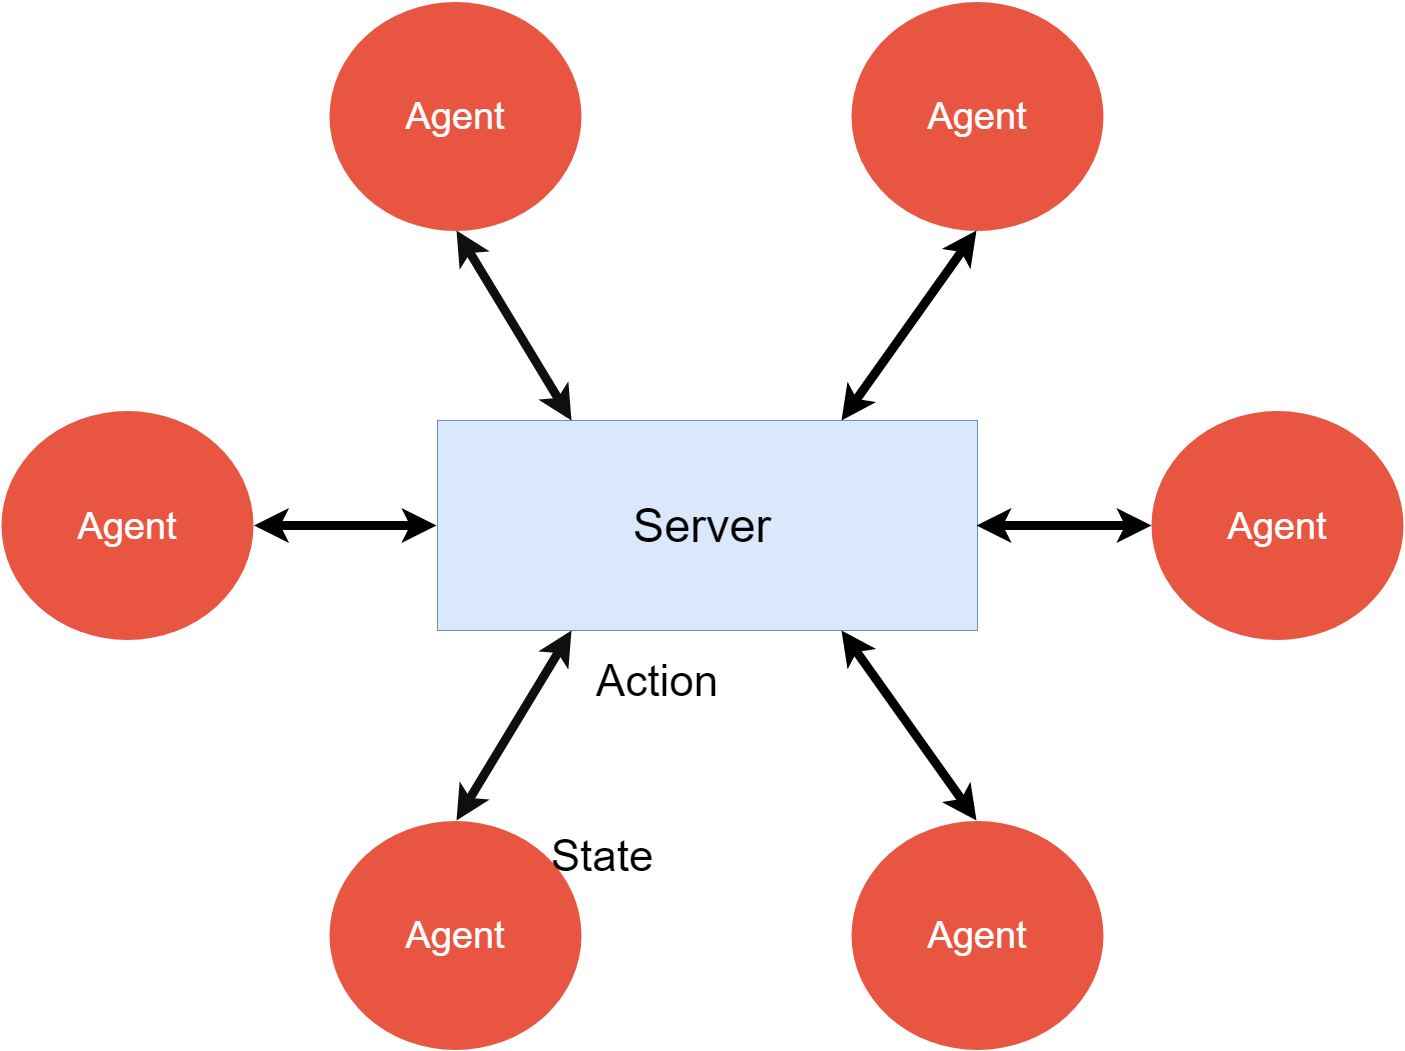
\includegraphics[width=0.6\textwidth]{Cap2/ServerAgent.png}
	\caption{Simple server-agent interaction diagram}
	\label{ServerAgent}
\end{figure}

\section{Physical model of rcssserver}

Here is described how the physical model of the  environment operates.

\subsection{Movement of the object}

When rcssserver's simulation cycle is updated, information on object movement is
updated in the following order.

\begin{enumerate}
	\item The acceleration of the agents are corrected so they do not overflow their respective maximum acceleration value.
	\item Add the acceleration vector to  velocity vector.
	\item The velocity of the agents are corrected so they do not overflow their respective maximum velocity value.
	\item Add noise to velocity vector.
	\item Check collision with goal post.
	\item Add velocity vector to  position vector.
	\item Decay speed
	\item Set the acceleration to zero.
	\item After updating all objects position, check for collisions.
\end{enumerate}

The position and speed will be updated in this procedure for both the ball and the
player.



\section{Player Model}

\subsection{Available Action Commands}
When the player agent makes a decision, it sends the action command necessary to realize  the  action  to  rcssserver,  rcssserver  accepts  the  following  commands  as player's actions.

\begin{table}
\caption{Agent possible actions}
\label{AgentActions}

\center
\begin{tabular}{cc}
  % after \\: \hline or \cline{col1-col2} \cline{col3-col4} ...
  \hline
	Action & Description   \\
	\hline
    kick  & Accelerate the ball in any direction.  \\
    dash  & Accelerate yourself toward the body.\\
	turn  & Rotate the direction of the body.\\
	tackle& Accelerate the ball toward the body.\\
	catch & (Only keeper) Catch the ball by hand.\\
	move  & Move instantaneously to the specified position.\\
	\hline
\end{tabular}
\end{table}

These commands move the body of the player agent.The command to move the body can be exclusively executed once per cycle, for example, when the rcssserver accepts the kick command from the player, the cycle ends That player will not be able  to  execute  the  new  body  moving  command  until  you  can  not  move  it diagonally because you can not use dash and turn at the same time.In addition the following auxiliary action command can be used.

\begin{table}
	\caption{Agent possible auxiliary actions}
	\label{AgentAuxiliaryActions}
	
	\center
	\begin{tabular}{cc}
		% after \\: \hline or \cline{col1-col2} \cline{col3-col4} ...
		\hline
		Auxiliary Action & Description   \\
		\hline
		turn neck  & Rotate the neck and change the direction of vision.  \\
		change view  & Change the viewing mode.\\
		turn  & Generate a communication message.\\
		say & Point to a specific position.\\
		point to & Pay attention to communication from specific players.\\
		\hline
	\end{tabular}
\end{table}

\section{The Penalty Event}
In the case of a tie, the match may be decided by penalty shootouts. In this event, an agent is set at a certain distance from the goal under possession of the ball while the keeper start at the goal line. After a trigger start, the attacker and the keeper may move and act freely, different from the real soccer game where in the penalty shootout event the shooter may only shoot and the keeper may only move above the goal line. So the possible actions the keeper may take are: \textit{dash} , \textit{turn} and \textit{catch} and the auxiliary action \textit{turn neck}